\RequirePackage{lineno} 
\documentclass[11pt,twoside,a4paper]{article}
\usepackage{graphicx,epsfig}
\usepackage{hhline}
\usepackage{booktabs}

\usepackage{amsmath,amssymb}
\usepackage{times}
\usepackage[varg]{txfonts}
\DeclareMathAlphabet{\mathbold}{OML}{txr}{b}{it}

\usepackage{array,multirow,dcolumn}
%\usepackage[mathlines,displaymath]{lineno}
\usepackage{rotating}

\usepackage[hypertexnames,setpagesize,%
    pdftex,%
    colorlinks,%
    citecolor=blue,%
    hyperindex,%
    plainpages=false,%
    bookmarksopen,%
    bookmarksnumbered%
  ]{hyperref}

% --- DO NOT remove this line:
\providecommand\texorpdfstring[2]{#1}

% we use natbib instead of cite to work with hyperref
%\usepackage{cite}
\usepackage[numbers,square,comma,sort&compress]{natbib}
%\usepackage{hypernat}
\usepackage{textcomp}

%\bibliographystyle{unsrt}
\bibliographystyle{writeup}
\renewcommand{\topfraction}{1.0}
\renewcommand{\bottomfraction}{1.0}
\renewcommand{\textfraction}{0.0}

% \renewcommand{\arraystretch}{1.2}
\newlength{\dinwidth}
\newlength{\dinmargin}
\setlength{\dinwidth}{21.0cm}
\textheight24cm \textwidth16.0cm
\setlength{\dinmargin}{\dinwidth}
\setlength{\unitlength}{1mm}
\addtolength{\dinmargin}{-\textwidth}
\setlength{\dinmargin}{0.5\dinmargin}
\oddsidemargin -1.0in
\addtolength{\oddsidemargin}{\dinmargin}
\setlength{\evensidemargin}{\oddsidemargin}
\setlength{\marginparwidth}{0.9\dinmargin}
\marginparsep 8pt \marginparpush 5pt
\topmargin -42pt
\headheight 12pt
\headsep 30pt \footskip 32pt
\parskip 3mm plus 2mm minus 2mm

\include{latex-defs}

\title{ \vspace{1cm} {\Huge HAverager } \\
              Data combination package  \\ 
              \vspace{0.5cm}
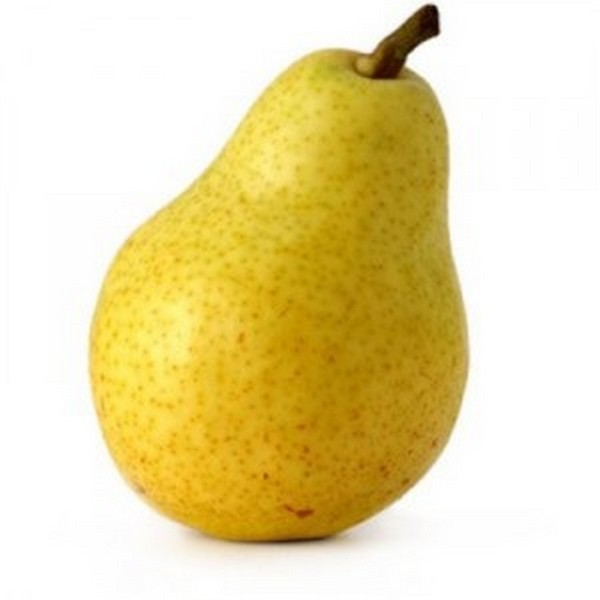
\includegraphics[width=0.25\linewidth]{figures/logo.jpg}}
\author{HAverager developers}
\begin{document}
\maketitle
\vspace{4cm}
\begin{abstract}
\vspace{0.5cm}
The presented stand-alone tool is designed to combine the data of the measurements. The combination process is based on the $\chi^2$ minimization with respect of the correlation model, assigned to uncertainties of the data points. The program performs a study of behaviour of the data-point uncertainties and tests the compatibility of the measurements. 
% The package is available for downloads on the web-site {\tt https://wiki-zeuthen.desy.de/HERAverager}
\end{abstract}
\thispagestyle{empty}
\newpage
\tableofcontents
\linenumbers
\newpage


\section{Introduction}

If two ore more measurements of the same physics quantity are statistically independent they can be combined to an average measurement. When these measurements have only one uncertainty and no information about correlation is known weighted-average algorithm can be used to calculated average value. However in many cases measurements are binned and performed with several sources of the correlated and uncorrelated systematic uncertainties. Presented package is designed in order to study the compatibility and perform bias-free combination of these measurements.

The combination procedure is based on the $\chi^2$ minimization. This package was originally developed for combination of two data sets of the H1 data~\cite{H1Comb} and then used for combination of data from two HERA experiments: H1 and ZEUS~\cite{HERAComb}. Currently this package is widely used for combination of LHC data.

Following types of the data-uncertainties are considered in presented tool:
\begin{itemize}
\item Statistical uncertainties. Usually based on square root of number of measured events. Uncorrelated between data sets and between bins.
\item Systematic uncertainties uncorrelated between bins. Can be correlated or uncorrelated between data sets.
\item Bin-to-bin correlated systematic uncertainties. Can be correlated or uncorrelated between data sets.
\begin{itemize}
\item Additive: not proportional to the measured values.
\item Multiplicative: proportional to the measured values.
\item Off-set: does not have any contribution to the $\chi^2$ and therefore does not have any impact on the average value.
\end{itemize}
\end{itemize}
Tool support asymmetric uncertainties.
 
This manual describe a linear $\chi^2$ definitions (see Sec.~\ref{Sec:Basic}) and explains the basic liner-algebra manipulations in Sec.~\ref{Sec:minimization}, which stays behind the combination procedure. Several different biases are discussed in Secs.~\ref{Sec:MultBias}--\ref{Sec:StatBias}. Bias-correction procedure introduces non-linear $\chi^2$, which minimized using linear approximation and iterative procedure is shown in Sec.~\ref{Sec:MinimizeBias}.

User manual describes the installation procedure (Sec.~\ref{Sec:Install}) and code description (Sec.~\ref{Sec:Code}). The input and output of the combination are discussed in Secs.~\ref{Sec:Input} and \ref{Sec:Output} respectively.  
\section{Combination method}
\label{sec:combDetails}

\subsection{Basic principal of the combination}
\label{Sec:Basic}
For a measurement $\mu$ with uncertainty $\Delta$, assuming a Gaussian shape of the uncertainty, the measurement can be considered as a probability distribution function for a ``true'' quantity $m$:
\begin{equation}
  P(m)=\frac{1}{\sqrt{2\pi \Delta}}\exp\left(-\frac{(m-\mu)^{2}}{2\Delta^{2}}\right)
  \label{Eq:PDFMeas}
\end{equation}
This can be written as a $\chi^2$ function by taking $-2\log$ (constant term was skipped):
\begin{equation}
  \chi^{2}(m)=\frac{\left( m-\mu  \right)^{2}}{\Delta ^{2}}
  \label{Eq:ChiSq1}
\end{equation}

Minimum of $\chi^2$ corresponds to $m=\mu$, while the change $\Delta \chi^2=1$ corresponds to $m=\mu \pm \Delta$. In case of two statistically independent measurements of the case quantity $m$: $\mu_1$, $\Delta_1$ and $\mu_2$, $\Delta_2$, the probability distribution function of $m$ is given by the  product of two:
\begin{equation}
P(m) \sim \exp \left( -\frac{(m-\mu_1)^2}{2\Delta_1^2} \right) 
\exp\left( -\frac{(m-\mu_2)^2}{2\Delta_2^2} \right),
\end{equation}
which corresponds to $\chi^2$ that is given by the sum of the two: $\chi^2_{sum} = \chi^2_1 + \chi^2_2$.

Since $\chi^2_{sum}$ is a positive definite quadratic form it can be re-written in the form of Eq.~\ref{Eq:ChiSq1}. In this case $\mu$ is replaced by average $\mu_{ave}$ and $\Delta$ is replaced by the error on this average:

\begin{equation}
  \chi^{2}(m)=\frac{ ( m-\mu_{ave} )^{2}}{\Delta^{2}_{ave}} + \chi^2_0,
  \label{Eq:ChiSum}
\end{equation}
where the value of $\chi^2_0$ measures consistency of the measurements, $\chi^2/N_{DoF}\sim 1$ for consistent measurements.

The value of $\mu_{ave}$ can be found by minimizing $\chi^2_{sum}$ with respect to $m$ (this leads to a usual averaging rule, $1/\Delta^2$ weights).


Many experiments measures a number of independent quantities $\mu_i$ which correspond to the underlying physics values $m_i$ (e.g. cross-section measurement in bins of $p_{T,Z}$, where $i$ refers to a bin number). In this case the $\chi^2$ function is a simple sum over the
measurements (bins):

\begin{equation}
  \chi^{2}_{exp}(m_i)= \sum_i \frac{ ( m_i-\mu_i )^{2}}{\Delta^{2}_i} + \chi^2_0,
  \label{Eq:ChiExp}
\end{equation}
Where:
\begin{itemize}
\item $\mu_i$ - the measurement in the bin $i$
\item $m_i$ ``truth'' value in the bin $i$~\footnote{Just to avoid confusion: ``truth'' here does not refers to MC-truth. This refers to a value, which we want to measure in experiment.}
\item $\Delta_i$ statistical uncertainty in bin $i$
\end{itemize}

The systematic effects, which affects the measurement $\mu_i$, are often correlated across bins. Let's consider measurement binned in a certain variable, which is affected by up/down shift of certain parameter:
\begin{equation}
  \mu_i \to \mu_i + \Gamma_i^+, \; \; \mu_i \to \mu_i - \Gamma_i^-, 
  \label{Eq:Systematics}
\end{equation}
where $\Gamma^{\pm}_i$ correspond to the variation up/down.

If the correlated systematic uncertainty is approximately symmetric, one can symmetrize them. For presented analysis following way was used:
\begin{equation}
\Gamma_i = max(|\Gamma_i^+|, |\Gamma_i^-|) \frac{\Gamma_i^+}{|\Gamma_i^+|},
  \label{Eq:Symmetrization}
\end{equation}
i.e. the size of the uncertainty is taken as maximal of up and down variations and the sign from one of the variations.

The symmetrised correlated systematic uncertainties were included into the $\chi^2$ function.

Systematic uncertainties, like energy scale, can be also viewed as a result of an experiment (e.g. measurement of the calibration): there is a ``true'' detector energy scale $\alpha$, measured detector calibration $\alpha_0$ and its statistical uncertainty $\Delta_{\alpha}$. Therefore, it is natural to add term
\begin{equation}
\chi^2_{syst}(\alpha) = \frac{(\alpha-\alpha_0)^2}{\Delta_{\alpha}^2}
  \label{Eq:ChiSyst}
\end{equation}
to the $\chi^2$ function. The nuisance parameter $b$, defined as  $b=(\alpha-\alpha_0)/\Delta_{\alpha}$ corresponds to a coherent change of measurements $\mu_i \to \mu_i + b\Gamma_i$. This defines the combined $\chi^2$ function:

\begin{equation}
  \chi^2(\vec{m},\vec{b})_{exp} = \sum_{i} \frac{(m_i-\mu_i-\sum_j \Gamma_i^j b_j)^2}{\Delta_i^2} + \sum_{j}
  b_j^2,
  \label{Eq:CorrChiSq}
\end{equation}
where
\begin{itemize}
\item $\vec{b}$ defines a vector of nuisance parameters $b_j$ corresponding to each source of systematic uncertainty,
\item summation over $i$ runs over all data points, and summation over $j$ runs over all correlated sources of systematic uncertainty,
\item $\Gamma_i^j$ is the absolute correlated systematic uncertainty, 
\item $\Delta_i$ is the uncorrelated (statistical) uncertainty.
\end{itemize}
With this definition minimum $\chi^2$ is obtained for all $m_i = \mu_1$ and $b_j=0$. If $b_j=0$ for all $j$ except $j=k$, $b_k=1$, then $\chi^2$ minimum is archived at $m_i = \mu_i + \Gamma_i^k$ and it is equal to 1.

Total uncertainty for a parameter $m_i$ defined by $\Delta \chi^2_{exp} = 1$ rule corresponds to the sum of correlated and uncorrelated uncertainties in quadrature: $\Delta^2_{i, tot} = \Delta^2_i + \sum (\Gamma^j_i)^2$.

\subsection{$\chi^2$ minimization}
\label{Sec:minimization}
Average of two data sets with systematic uncertainties follows the same ideas as for average of uncorrelated measurements: represent the sum of two $\chi^2$ by a single $\chi^2$:
\begin{equation}
  \chi^2(\vec{m_1},\vec{b_1})_{exp,1} + \chi^2(\vec{m_2},\vec{b_2})_{exp,2} =
  \chi^2_0 + \chi^2(\vec{m_{ave}},\vec{b'_{ave}}).
\end{equation}
The dimension of $\vec{m_{ave}}$ is equal to dimension of union set of $\vec{m_1}$ and $\vec{m_2}$. e.g. if both experiments measure for the same binning, $N_{M1} = N_{M2} = N_{M,ave} = N_M$. Similarly, for the systematic uncertainties $N_{S,ave} = N_{S1} + N_{S2} - N_{S, common} = N_S$, where $N_{S, common}$ is the number of common systematic error sources for the two measurements.

More explicitly, the sum of two $\chi^2$:
\begin{equation}
  \chi^2(\vec{m},\vec{b})_{sum} = \sum_e \sum_{i}^{N_M} \frac{ \left(m_i-\mu_{i,e}-\sum_j^{N_S} \Gamma_{i,e}^j b_j \right)^2}{\Delta_{i,e}^2} W_{i,e} + \sum_{j}^{N_S} b_j^2,
  \label{Eq:Chi2SumExp2}
\end{equation}
where,
\begin{itemize}
\item $i$ runs over all measured points $N_M$
\item $j$ runs over all sources of systematic uncertainties $N_S$
\item symbol $W_{i,e}$ is equal to 1 if data set $e$ contributes to a measurement at the point $i$, otherwise it is 0.
\item $\Gamma^i_{j,e}$ equals to 0 if the measurement $i$ from the data set $e$ is insensitive to the systematic source $j$.
\end{itemize}
This definition of $\chi^2$ assumes that the data sets $e$ are statistically uncorrelated. The systematic error sources $b_j$, however, may be either uncorrelated (separate sources) or correlated across data sets (different data sets sharing a common source).

Since $\chi^2_{sum}$ is a quadratic form of $\vec{m}$ and $\vec{b}$, it may be rearranged such that it takes a form similar to Eq.~\ref{Eq:ChiSum}.
\begin{eqnarray}
  \chi^2(\vec{m},\vec{b}) = \chi^2_{min}  + \sum_{i}^{N_{M,ave}} \frac{ \left(m_i-\mu_{i,ave}-\sum_j^{N_{S,ave}} \Gamma_{i,ave}^j (\alpha_j-\alpha_{j,ave}) \right)^2}{\Delta_{i,ave}^2} + \nonumber \\
+ \sum_{j}^{N_{S,ave}} \sum_{k}^{N_{S,ave}} (\alpha_j-\alpha_{j,ave})(\alpha_k-\alpha_{k,ave})(A_S')_{ik},
  \label{Eq:ChiBefore}
\end{eqnarray}
where
\begin{itemize}
\item $\mu_{i,ave}$ are average values of measured quantities
\item $\Delta_{i,ave}$ are their uncorrelated uncertainties
\end{itemize}

The values of $\alpha_{j, ave}$, $\Delta_{i,ave}$, $\mu_{i,ave}$ and matrix $A_{S}'$ are determined by minimization of $\chi^2$ function in Eq.~\ref{Eq:Chi2SumExp2} with respect to $m_i$ and $b_j$. The minimum of Eq.~\ref{Eq:Chi2SumExp2} is found by solving a system of linear equations obtained by requiring $\partial \chi^2 / \partial m_i = 0$ and $\partial \chi^2 / \partial b_j = 0$ which can be written in matrix form
\begin{equation}
\begin{pmatrix}
A_M & A_{SM} \\
(A_{SM})^T & A_S \\
\end{pmatrix}
\begin{pmatrix}
M_{ave} \\
B_{ave} \\
\end{pmatrix}
=
\begin{pmatrix}
C_M \\
C_S \\
\end{pmatrix}
\label{Eq:MatrixEQ}
\end{equation}
where
\begin{itemize}
\item vector $M_{ave}$ corresponds to all measurements
\item vector $B_{ave}$ corresponds to all sources of the systematic uncertainties
\item matrix $A_M$ has a diagonal structure with $N_{M,ave}$ diagonal elements $A_{M}^{ii} = \sum_e \frac{W_{i,e}}{\Delta^2_{i,e}}$
\item $A_{SM}^{ij} = - \sum_e \frac{\Gamma^j_{i,e}}{\Delta^2{i,e}} W_{i,e}$
\item $A_S^{ij} = \delta_{ij} + \sum_e \sum_k^{N_M} 
\frac{ \Gamma^k_{i,e} \Gamma^k_{j,e}}{\Delta^2_{k,e}} W_{k,e}$
\item $C_M^i = \sum_e \frac{\mu^i_e}{\Delta^2_{i,e}} W_{i,e} $
\item $C_S^j = -\sum_e \sum_k^{N_M} \frac{\mu^k_e \Gamma^k_{j,e}}{\Delta^2_{k,e}} W_{k,e}$
\end{itemize}
Here $\delta_{ij}$ is the Kronecker symbol. The matrix $A_{SM}$ has dimension $N_M \times N_S$ while the matrix $A_S$ is quadratic with $N_S \times N_S$ elements.

Using the method of the Schur complement, the solution is found as:
\begin{eqnarray}
A_S' = A_S - (A_{SM})^T A_M^{-1} A_{SM} \nonumber  \\
B_{ave} = (A_S')^{-1} (C_S - (A_{SM})^T A_M^{-1} C_M) \nonumber  \\
M_{ave} = A_M^{-1} (C_M - A_{SM} B_{ave})
\end{eqnarray}
Given the components of the vector $B_{ave}$,  $\beta_{j, ave} = \alpha_{j,ave}/\Delta_{\alpha_j}$, the solution for $\mu_{i, ave}$ can be written in explicit form:
\begin{equation}
\mu_{i, ave} = \frac{\sum_e \left(\mu_{i,e} + \sum_j \Gamma^i_{j,e} \beta_{j,ave} \right)
\frac{W_{i,e}}{\Delta^2{i,e}} }{\sum_e \frac{W_{i,e}}{\Delta^2_{i,e}}}
\label{Eq:AveMu}
\end{equation}
The uncorrelated uncertainty squared is determined by the inverse of the elements of the diagonal matrix $A_M$:
\begin{equation}
\Delta^2_{i,ave} = \frac{1}{\sum_e \frac{W_{i,e}}{\Delta^2_{i,e}}}
\label{Eq:AveDelta}
\end{equation}

Eq.~\ref{Eq:AveMu} and \ref{Eq:AveDelta} reproduce the standard formula for a statistically weighted average of several uncorrelated measurements when all shifts of the systematic error sources are set to zero. The values of $\beta_{i, ave}$ in Eq.~\ref{Eq:AveMu} show, how the combined measurements $\mu_{i, ave}$ are shifted, compared to initial measurements $\mu_{i,e}$ in terms of systematic uncertainties $\Gamma^j_{i,e}$.

The non-diagonal nature of the matrix $A_S'$ expresses the fact that the original sources of the systematic uncertainties are correlated with each other after averaging. The matrix $A_S'$ can be decomposed to re-express Eq.~\ref{Eq:CorrChiSq} in terms of diagonalised sources of systematic uncertainties:
\begin{equation}
DD = UA_S' U^{-1} \; \; \; \Gamma_{ave} = A_{SM} A_M^{-1} D^{-1} U^{-1}
\label{Eq:Diag}
\end{equation}
Here $U$ is an orthogonal matrix composed of the eigenvectors of $A_S'$, $D$ is a diagonal matrix with corresponding square roots of eigenvalues as diagonal elements and $\Gamma_{ave}$ represents the sensitivity of the average result to these new sources. Its elements are the $\Gamma_{i,ave}^j$.

After diagonalizability of matrix $A_S'$, $\chi^2$ function in Eq.~\ref{Eq:ChiBefore} can be re-written in form, similar to Eq.~\ref{Eq:CorrChiSq}:

\begin{equation}
  \chi^2(\vec{m},\vec{b'})_{tot} = \chi^2_{min} + 
  \sum_{i}^{N_M} \frac{(m_i-\mu_{i,ave}-\sum_j^{N_S} \Gamma_{i,ave}^j b_j')^2}{\Delta_{i,ave}^2} + \sum_{j}^{N_S}  (b_j')^2,
\label{Eq:ChiAfter}
\end{equation}
where $b'_j = \sum_k U_{jk}(b_k - \beta_{k,ave})D_{jj}$.

The orthogonal matrix $U$ connecting the systematic sources before and after averaging with Eq.~\ref{Eq:Diag}. Diagonal elements of matrix $D$ shows, how the uncertainties of combined measurement $\Gamma^j_{i,ave}$ are reduced, compared to initial systematic uncertainties.

The value of $\chi^2_{min}$ corresponds to the minimum of Eq.~\ref{Eq:Chi2SumExp2} and calculated using values of $\mu_{i, ave}$ and $\beta_{j, ave}$ as a parameters $\vec{m}$ and $\vec{b}$. The ratio $\chi^2_{min}/N_{DoF}$ is a measure of the consistency of the
data sets. The number of degrees of freedom, $N_{DoF}$, is calculated as the difference between the total number of measurements and the number of the measured points $N_M$. It is useful to note, the definition of $\chi^2_{min}$ have two contributions, one is a usual shift if the measurement weighted with uncorrelated uncertainties (comes from $\mu_{i, ave} - \mu_{i,e}$). Another contribution comes from correlated uncertainty term. %This procedure represents a method to average data sets, which allows correlations among the measurements due to systematic uncertainties to be taken into account.

Another interesting parameter, which shown the compatibility of channels is pull of the central values:
\begin{equation}
p^{i,e} = \frac{\mu^{i,e} - \mu^{i,ave}(1 - \sum_j\gamma_{i,e}^j\beta_{j,ave})}{\sqrt{\Delta^2_{i,e}-\Delta^2_{i,ave} } },
\label{Eq:Pulls}
\end{equation}
where $\gamma^j_{i,e} = \Gamma^j_{i,e} / \mu_{i,ave}$. This definition is similar to the $\chi^2$ definition, but not summed over bins. These pulls show how the average measurement are shifted compare to individual measurement and also have two contributions, similar to $\chi^2$.

The values, which reflect only correlated part are the shifts $\beta$. If the systematic uncertainties for measurement have rather similar size, than average fluctuation of shifts will reflect the correlated contribution to $\chi^2$ compatibility. However we can always add such uncertainties to analysis, which will be not shifted after combination and therefore will just make smaller average fluctuation of shifts. Large shifts indicates, that corresponding central value of the systematic uncertainties were initially not correctly estimated (and therefore shifted during the combination).

The values coming out of matrix $D$ show, how much the initial systematic uncertainties were reduced due to the combination. This parameter does not directly related to the channel compatibility, but show how much we gain out of the combination. 

The pull for systematic uncertainties can be defined as:
\begin{equation}
p^{i} = \frac{\beta_{i,ave}}{\sqrt{1 - D_{ii}^2} }.
\label{Eq:PullSyst}
\end{equation}
This value shown, how significant was the systematic shifted due to the combination. The large systematic pull suggests, that systematic uncertainty was not correctly estimated.

\subsection{Covariance matrix representation of the systematic uncertainties}
\label{sec:decomposition}
Another way representing bin-to-bin (point-to-point) correlations is by using a covariance matrix $C$:
\begin{equation}
\chi^2(\vec{m}) = \sum_{ik}^{N_M} (m_i-\mu_i)^T C_{ik}^{-1} (m_k-\mu_k), \; 
C_{ik} = \sum_{j}^{N_S}\Gamma^j_i \Gamma^j_k,
\label{Eq:ChiCovar}
\end{equation}
where $N_M$ is a number of bins and $N_S$ is a number of cources of the systematic uncertainties. For Gaussian uncertainties covariance matrix and nuisance parameter representations are equivalent.

Matrix $C$ can be written as:
\begin{equation}
C_{ik} = \sum_{lj}^{N_M} G^{-1}_{il} D_{lj} G_{jk},
\label{Eq:Decomposition}
\end{equation}
where columns of $G^{-1}$ are made of eigenvectors of $C$, sorted by eigenvalues (largest to smallest) and $D$ is a diagonal matrix made of the eigenvalues of $C$.

Since $C$ is positively defined, the eigenvalues are real and grater zero and we can assume $G' = \sqrt{D}G$. Also $G^{-1} = G^T$, since $G$ is the orthogonal and then
 \begin{equation}
C_{ik} = \sum_{j}^{N_M} G_{ij}^{'T} G_{jk}'.
\end{equation}

The contribution of eigenvectors with small eigenvalues can be neglected by truncating the sum after $N_S' < N_S$.
\begin{equation}
C_{ik} \approx C'_{ik} = \delta_{ik}\Delta^2_{i, uncorr} + \sum_{j=1}^{N_S'} G'^T_{ij}G'_{jk}, \;\;
\Delta^2_{i, uncorr} = \sum_{j=N_S'+1}^{N_M} (G'_{ij})^2.
\end{equation}
Here $\delta_{ik}$ is the Kronecker symbol and  $\Delta_{i, uncorr}$ is uncorrelated systematic uncertainty. To preserve the total uncertainty, $\Delta_{i, uncorr}$ are chosen such, that diagonal elements in $C'$ are equal to the diagonal elements in $C$. The dimension $N_M$ of covariance matrix $C'$ is not reduced by this approximation. 

The reduced summation allows for more compact representation using nuisance parameters. The 
$\chi^2$ function takes form:
\begin{equation}
  \chi^2(\vec{m},\vec{b})_{exp} = \sum_{i} \frac{(m_i-\mu_i-\sum_j \Gamma_i^j b_j)^2}{\Delta_{i, stat}^2 + \Delta_{i, uncorr}^2} + \sum_{j}
  b_j^2,
  \label{Eq:CorrChiSq2}
\end{equation}


\subsection{Bias correction for multiplicative uncertainties}
\label{Sec:MultBias}
Many of the systematic uncertainties for the data measurements, correlated and uncorrelated are multiplicative, e.g. they are proportional to the measured values.

Consider two measurements $\mu_1$ and $\mu_2$ of $m$. Let's assume, that $\mu_1 = m + mb$, $\mu_2 = m-mb$. Both measurements are performed with the same relative uncertainty $\delta$. An error weighted average of the two measurements returns

\begin{equation}
  \mu_{ave} = m \frac{1-b^2}{1+b^2},
  \label{Eq:ErrorAverage}
\end{equation}
which for $b=5\%$ corresponds to 0.5\% bias.

The bias occurs because the measurement at smaller value $\mu_2$ got smaller absolute uncertainty $\delta(m-mb)$.

Measurements with multiplicative uncertainties can be combined bias-free using
expected values $m_i$ instead of measured $\mu_i$ to translate relative to absolute uncertainties. In this case Eq.~\ref{Eq:CorrChiSq} takes form:

\begin{equation}
  \chi^2(\vec{m},\vec{b})_{exp,mult} = \sum_{i} \left(\frac{m_i[1-\sum_j \gamma_i^jb_j]  - \mu_i}{\delta_{i}m_i}\right)^2 + \sum_{j}  b_j^2,
  \label{Eq:StatCorrChiSq2a}
\end{equation}

\subsection{Bias correction for statistical uncertainties}
\label{Sec:StatBias}
Let's consider the counting of number of arbitrary events. Two measurements $\mu_1$ and $\mu_2$ gives $\mu_1 = N_1$, $\mu_2 = N_2$. Statistical uncertainties of the measurement are estimated as a square root of number of counts. Weighted average for these measurement returns:

\begin{equation}
  \mu_{ave} = \frac{2N_1N_2}{N_1+N_2},
\end{equation}

instead of 

\begin{equation}
  \mu_{ave} = \frac{N_1 + N_2}{2}
\end{equation}

Bias for statistical average can removed by using expected instead of measured number of events. If statistical uncertainty for a measurement is quoted based on square root of number of measured events, then estimated unbiased relative statistical uncertainty $\delta_{stat,cor} = \frac{\sqrt{m}}{\mu} = \delta_{stat} \sqrt{\frac{m}{\mu}} $. Absolute unbiased statistical uncertainty can be expressed as:

\begin{equation}
 \Delta_{stat,cor} = \delta_{stat} \sqrt{m\mu}
  \label{Eq:StatCorr}
\end{equation}

Finally, the number of observed events can be modified by the correlated systematic uncertainties. This modification can be taken into account by using 
\begin{equation}
  m(1-\sum_j \gamma^jb_j)
  \label{Eq:StatCorr2}
\end{equation}
instead of $m$ in Eq.~\ref{Eq:StatCorr}. This brings us to the $\chi^2$  formula:

\begin{equation}
  \chi^2(\vec{m},\vec{b})_{exp,cor} = \sum_{i} \frac{(m_i[1-\sum_j \gamma_i^jb_j]  - \mu_i)^2}{\delta_{i, stat}^2\mu_im_i[1-\sum_j \gamma_i^jb_j] + \delta_{i, uncorr}^2m_i^2} + \sum_{j}
  b_j^2,
  \label{Eq:StatCorrChiSq2b}
\end{equation}


\subsection{Treatment of off-set systematic uncertainties}
\label{Sec:offset}

Let's consider a source of systematic uncertainty on a certain measurement (so called off-set systematics), which does not have any contribution to the $\chi^2$ and therefore does not have any impact on the average value. Systematic uncertainty on the combined value due to this source ($\delta^{off-set}_{ave}$) can be calculated as: 

 \begin{equation}
  \delta^{off-set}_{ave} = \frac{\mu_{ave}^{up} - \mu_{ave}^{down}}{\mu_{ave}},
\end{equation}
where $\mu_{ave}^{up/down}$ the average value of the measurements $e$, shifted by considered off-set systematics $\mu_e \pm \delta^{off-set}$. Therefore in case of $N_o$ sources of the off-set systematics combination procedure performs $2N_o+1$ times: one nominal combination, $N_o$ ``up'' and $N_o$ ``down'' combinations for each sources of the off-set systematic respectively.


\subsection{Treatment of asymmetric systematic uncertainties}
\label{Sec:AsymmUncert}

In case if assumption of the symmetric systematic uncertainty (expressed by Eq.\ref{Eq:Symmetrization}) is not valid for performed measurement, the $\chi^2$ Eq.~\ref{Eq:CorrChiSq} can be written in more general form:

\begin{equation}
  \chi^2(\vec{m},\vec{b})_{exp} = \sum_{i} \frac{(m_i-\mu_i-\sum_j f_i(b_j))^2}{\Delta_i^2} + \sum_{j} b_j^2.
  \label{Eq:CorrChiSq3}
\end{equation}
If $f_i(b_j) = \Gamma_i^jb_j$,  Eq.~\ref{Eq:CorrChiSq3} again back to Eq.~\ref{Eq:CorrChiSq}. Asymmetric systematic uncertainties can be approximated as:

\begin{equation}
f_i(b_j) = \Gamma_i^jb_j + \omega_i^jb_j^2, \; \omega_i = \frac{\Gamma_i^{j+} + \Gamma_i^{j-}}{2}.
  \label{Eq:AsymmUnc}
\end{equation}
$\chi^2$ definition in this case become non-linear. Instead of simple minimization procedure described in Sec.~\ref{Sec:minimization}, iterative minimization procedure, shown in Sec.~\ref{Sec:MinimizeBias} is used. 

\subsection{Different representation of combined uncertainties}
\label{Sec:SystRepresentation}

The systematic uncertainties of the averaged values are presented in orthogonal way (in terms of diagonalised sources of systematic uncertainties) by $\Gamma_{ave}$ (see Eq.\ref{Eq:Diag}). However in this representation each sources of the systematic uncertainty $\Gamma_{ave}^j$ is a linear combination of the initial sources of the systematic uncertainties $\Gamma^j$.  

In order to be able to compare systematic uncertainties of the combined measurement with $\Gamma^j$ source by source, diagonal elements of matrix $A_S'$ can be taken as it is (without diagonalisation). However in this case systematic uncertainties of the combined measurement will be not orthogonal and their quadratic sum will not give a total systematic uncertainty.

Alternative way is to use half-diagonal form of matrix $A_S'$. In this case systematic uncertainties of the combined measurement are orthogonal, however one of the course corresponds to one of the sources on the initial systematic uncertainties $\Gamma^j$. 


\subsection{Combination with bias corrections}
\label{Sec:MinimizeBias}

For most practical situations the bias, described in Sec.~\ref{Sec:MultBias} and \ref{Sec:StatBias} of the average is small. Therefore, the expectation $m_i$ can be estimated in an iterative procedure starting from linear formula Eq.~\ref{Eq:CorrChiSq} and using $m_i = \mu_{i,ave}$. The key for the unbiased result is that the same expectation is used for all measurements. In most cases the convergence is observed after second iteration.

Similar iterative approach is applied to combine the measurements with asymmetric systematics uncertainties, introduces in Sec.~\ref{Sec:AsymmUncert}. The first iteration is performed with linearised $\chi^2$ Eq.\ref{Eq:CorrChiSq} using symmetrised uncertainties $\Gamma$ (linear part of $f(b_j)$). The next iterations are performed with corrected uncertainties $\Gamma' = \Gamma + \omega*\beta_{ave}$, e.g. correction depends on the systematic shift. The combination procedure require several iterations.

Described bias corrections and correction of the systematic uncertainties are not interfere with each other and therefore both are applied in simultaneously. E.g. at each iterations both bias corrections and correction for non-symmetric uncertainties are applied. 

Iterative averaging with bias correction and only symmetrical uncertainties converging fast and requires 2--3 iterations. Presence of asymmetric uncertainties make convergence worse. In some cases iterative procedure will not converge at all. In order to monitor convergence of the iterative procedure systematic shifts $\beta_{ave}$ for each iteration have to be considered.

\section{Program manual}
\label{Sec.FortranProgram}

This is Fortran-base open-source software, which can be downloaded from: {\tt https://wiki-zeuthen.desy.de/HERAverager}. Installation and basic pre-requirements are described in Sec.~\ref{Sec:Install}. Code organization is shown in Sec.~\ref{Sec:Code}.

The input and output formats are explained in Sec.~\ref{Sec:Input} and Sec.~\ref{Sec:Output} respectively.

\subsection{Program installation}
\label{Sec:Install}
The program requires gfortran compiler to be compiled.

The program can be unpacked and installed with following lines:
\begin{verbatim}
    tar -xvzf heraverager-1.0.0.tar.gz
    cd heraverager-1.0.0
    autoreconf --install
    ./configure
    make 
    make install
\end{verbatim}

After successful installation an executable file can be found in: {\tt ./bin/HERAverager }. All input parameters are defined in the steering file. Test run of the program, using test steering file (is in {\tt ./test/steering}) can be performed with lines:

\begin{verbatim}
    cd ./bin
    ./HERAverager ../test/steering
\end{verbatim}

The output information is located in {\tt ./output/}

\subsection{Code organization}
\label{Sec:Code}

Package consist of following subdirectories:

\begin{itemize}
\item {\tt include}: include-file with declaration of global variables
\item {\tt source}: source-code files
\item {\tt doc}: documentation to the program, including this manual.
\item {\tt test}: example of steering and data files
\item {\tt num\_utils}: Utilities for the averaging.
\end{itemize}

Short description of source files is given below:

\begin{itemize}
\item {\tt averaging.f}: Calling functions to prepare arrays and perform the combination   
\item {\tt average\_py.f90}: Interface to python (see Sec.~\ref{sec:python})
\item {\tt error\_logging.f}: print full error summary and close files
\item {\tt initave.f}: Reading the data and preparing for the combination
\item {\tt statrecalc.f}: Recalculate systematic uncertainties after combination and prepare values for the next iterator. 
\item {\tt common\_tools.f}: Function, used in different steps of the combination 
\item {\tt fillarrays.f}: Prepare arrays used for combination
\item {\tt output.f}: Print output of the combination in output files
%\item {\tt swimming.f}
\item {\tt covartonui.f}: Convert covariance matrix to nuisance param. representation
\item {\tt heraverager.f}: Main file, which is calling functions for initialization, combination and output.
\item {\tt readdata.f}: Read a table of measurement with their uncertainties from single experiment
\item {\tt toblockdiag.f}: Perform the combination by minimization of linearised $\chi^2$
\end{itemize}

Summary of the code structure is shown in Fig.~\ref{fig:code}. 3 logic blocks: initialization, combination and output are encapsulated in 3 functions called in {\tt heraverager.f}.

At initialization step all files with data and options are read and values are stored in global internal variables. First code read the steering file, which contain all options of the combination and list of data files. During the loop over data files the name of systematic sources, values of the measurements and their uncertainties are stored in global variables.

Combination block have a loop over all off-set systematics (2N+1 times, see Sec.~\ref{Sec:offset}) and over iterations. Combination process starts with filling of auxiliary arrays (mainly elements of Eq.~\ref{Eq:MatrixEQ}). Then minimization is performed and results are stored in global internal variables. In case if it was not the last iteration statistical and systematic uncertainties are recalculated (See Sec.~\ref{Sec:MinimizeBias}).

The output written in different files. Systematic uncertainties can be presented in different ways (See Sec.~\ref{Sec:SystRepresentation}), depending on options in the steering file.


\begin{figure}
  \centering
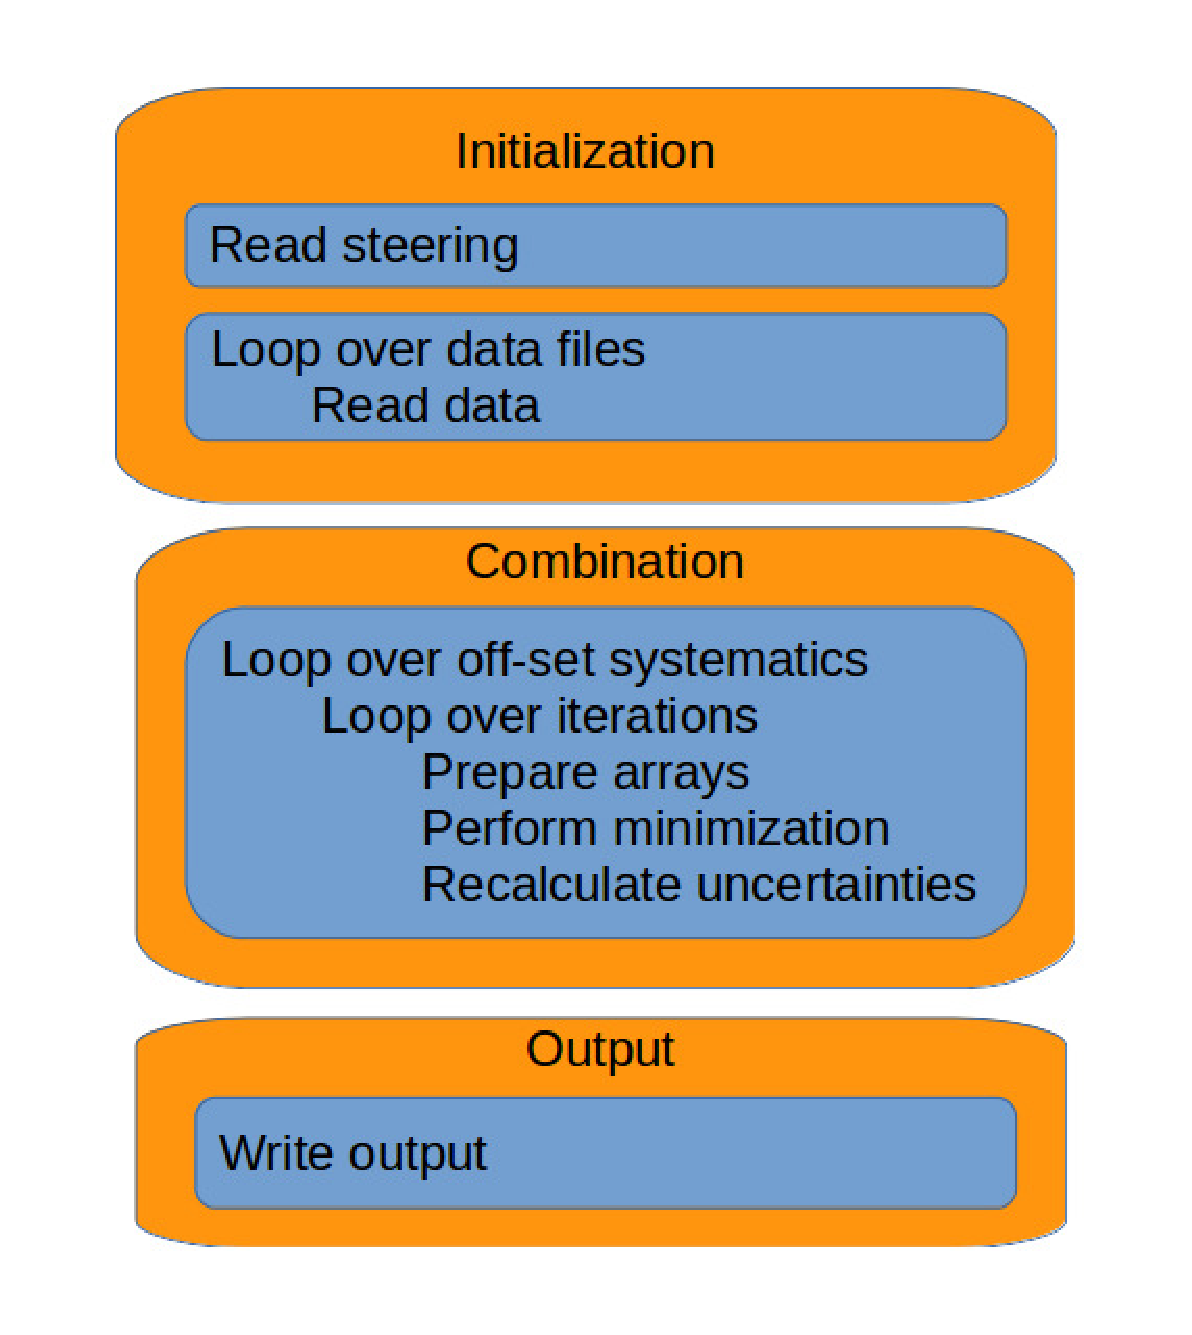
\includegraphics[width=0.65\linewidth]{figures/code.pdf}
  \caption{Code organization of the combination tool.}
  \label{fig:code}
\end{figure}


\subsection{Input information}
\label{Sec:Input}

All input of the combination as well as the list of data files and supplementary information is given in the steering file. The description of the steering file in given in Sec.~\ref{Sec:Steerign}, while data file is discussed in Sec.~\ref{Sec:Data}.

\subsubsection{Steering file}
\label{Sec:Steerign}

Steering file is organized in blocks, which corresponds to name-lists in the Fortran code. Lines, which starts with ! are commented. Structure and meaning of these blocks are described below:

\begin{verbatim}
&InFiles
  ! Specify data files to be averaged
  NInputFiles = 2
  InputFileNames(1) = '../test/h1460new.public.dat'
  InputFileNames(2) = '../test/zeus460.public.dat'
&End
\end{verbatim}
Block contains the list of data-files (see structure of the data files in Sec.~\ref{Sec:Data}). Path to these files have to be absolute and relative with respect to the place, where the program runs.


\begin{verbatim}
&CommonGrid
  GridType = 'External' !  'External' or 'Auto'
  GridFiles = '../test/grid460575.dat'
  AveSameExp = .true.
&End
\end{verbatim}
Most of the measurements, for which tool is designed are binned measurements. The binning can be taken directly from the data file (option {\tt 'Auto'}) or can be written externally (option {\tt 'External'}) in grid of bins. 

In case of external binning, files which describe binning have to be provided and have structure, similar to:

\begin{verbatim}
&Grid
  Reaction = 'NC e+-p'
  NDimension = 2
  NPoints = 630
  BinNames = 'Q2','x'
&End
  1.5  0.000378678
  1.5  0.000227206998
  1.5  0.000134258007
  1.5  9.52802002E-05
\end{verbatim}
Where:
\begin{itemize}
\item {\tt Reaction} is the name of measured process
\item {\tt NDimension} is the number of dimensions of the binning
\item {\tt NPoints} total number of bins
\item {\tt BinNames} name of the dimensions.
\end{itemize}

Numbers below the header define the center of bins. Each line represent one bin (number of lines should be equal to the total number of bins). Number of columns corresponds to the number of dimensions (two in this example) and define center of bins in each dimension ('Q2' and 'X' in example).

Each grid-file describe the binning for a certain measured process (reaction). In case of combination of the data for several different processes, several grid files have to be given.

The name of dimensions and the name of measured process should coincide with one given in data file (see Sec.~\ref{Sec:Data}). The measurements are considered as a measurements of the same physics quantity if bins, bin names and reactions are coincides. 

In case if the bin-centers in the data file are different compared to bin-centers in the grid file nearest bin of the grid file will be used to define the bin. Parameter {\tt AveSameExp} clarifies, how to treat the case when two bins from one experiment go to one grid bin:
\begin{itemize}
\item {\tt .true.} - weighted average of these bins will be used for combination.
\item {\tt .false.} - measurements in these bins will be combined as different measurements of the same physics quantity.
\end{itemize}

\begin{verbatim}
&HERAverager
  OutputMode  = 'ORTH'
  OutputPrefix = 'Ave' 
  OutputFolder = '../output'   
  IDebug = 0
  WriteOriginal = .false.
  WriteSysTexTable = .false.
  PostRotateSyst = .true.
&End
\end{verbatim}

{\tt OutputMode} - is the output options for the systematics uncertainties (see Sec.~\ref{Sec:SystRepresentation}).
\begin{itemize}
\item {\tt 'ORTH'} - orthogonal representation
\item {\tt 'ORIG'} - original structure of the systematic uncertainties.
\end{itemize}

{\tt OutputPrefix} Add a prefix for output file names

{\tt OutputFolder} - folder, where the output information is stored

{\tt PostRotateSyst = .true.} keep output systematic uncertainties align to the original sources as much as possible.

{\tt IDebug} - Debug level. Higher value corresponds to more debug messages.

{\tt WriteOriginal} - include original information to the output summary (file {\tt ave Ave.dat}, see Sec.~\ref{Sec:Output}) 

{\tt WriteSysTexTable} - write output information about systematic uncertainties in tex format (file {\tt sys.tex}, see Sec.~\ref{Sec:Output})

\begin{verbatim}
&BiasCorrection
  AverageType = 'MIXED'
  Iteration = 10
 ! Rescale the stat and uncorr uncertainties separately:
  RescaleStatSep = .false.
 ! Correction of the syst bias for stat errors
  CorrectStatBias = .false.
 ! Keeping the stat errors fixed'
  FixStat = .false.
&End
\end{verbatim}
Parameter {\tt AverageType} define the type of the systematic uncertainties
\begin{itemize}
\item {\tt 'ADD'} - all systematic uncertainties are processed as additive
\item {\tt 'MULT'} - all systematic uncertainties are processed as multiplicative
\item {\tt 'MIXED'} - type of systematic uncertainties is taken from the data file
\end{itemize}

Parameter {\tt Iteration} set the number of iterations. In case, if all uncertainties are additive and symmetric $\chi^2$ is linear, no additional iteration is required. In case of multiplicative systematic uncertainties 2-3 iterations are recommended to get stable combined value. If some of the uncertainties are asymmetric number of iteration have to increased (7-10 iterations).

Correction of the statistical uncertainties, discussed in Sec.~\ref{Sec:StatBias} is normally performed for both statistical and uncorrelated systematic uncertainties. This correction can be done separately for each of therm by setting flag {\tt RescaleStatSep = .true.}. Using flag {\tt FixStat = .false.} statistical uncertainties are still uncorrected.

Setting flag {\tt CorrectStatBias = .true.} statistical bias is corrected by implementing Eq.~\ref{Eq:StatCorr2}


\subsubsection{Data file}
\label{Sec:Data}

The data-file is an ascii-file, which contains measurement values in a certain bins and their uncertainties. 

The data file consist of the header and lines of data:
\begin{verbatim}
 &Data
   Name = 'H1' 
   NData = 72
   NColumn = 9
   ColumnType = 2*'Bin','Sigma', 6*'Error' 
   ColumnName = 'Q2', 'x', 'x-sec', 'stat', 'uncor','sys1','sys2:O','sys3+','sys3-'
   Reaction = 'NC e+-p' 
                                                     
   Percent = true,true,true,true,true,true
                                                     
 &END
   1.500  3.47999E-05  0.51952   8.10   4.96  0.69  8.00  0.45   0.58   
   2.000  4.64000E-05  0.70449   4.57   4.31  1.10 -0.81  0.49   0.59
\end{verbatim}

Header of the data file contain following information:

\begin{itemize}
\item {\tt Name}: A name of the data file, which is used for user-friendly output
\item {\tt NData}: Number of data points (bins)
\item {\tt NColumn}: Total number of columns in the table, which includes bins, value of the measurement and uncertainties
\item {\tt ColumnType}: Type of the column. In case if several columns have the same type they can be grouped as e.g. {\tt 6*'Error'}. All columns should have a type. Following types are supported:
\begin{itemize}
\item {\tt Bin}: Bin-center. Number of these columns gives the number of dimensions of the measurement.
\item {\tt Sigma}: Value of the measurement  
\item {\tt Error}: Uncertainty
%\item {\tt ignore}: column is ignored
\end{itemize}
\item {\tt ColumnName}: The name of the column. All columns should have a name. In case of 'Bin' type of the column name specify the name of the dimension. If case of using external grid file these names have to be mentioned in the grid file. For the 'Error' type of the column the name specify the name and type of systematic uncertainty. Following type of systematic uncertainties are supported:
\begin{itemize}
\item {\tt stat}: Statistical uncertainty
\item {\tt uncor}:  Bin-to-Bin uncorrelated systematic uncertainty
\item {\tt ignore}: Column ignored
\item {\tt somename}: Bin-to-Bin correlated multiplicative systematic uncertainty with the name ``somename''. One data-file should not contain two columns with uncertainties with the same names. If systematic uncertainty with the same name is found in different data-files, they are considered as correlated between measurements.
\item {\tt somename:O}: Off-set systematic uncertainty
\item {\tt somename:A}: Bin-to-Bin correlated additive systematic uncertainty
\item {\tt somename+}, {\tt somename-}: Bin-to-Bin correlated asymmetric systematic uncertainty (can be {\tt :0} or {\tt :A}). Each asymmetric systematic uncertainty should contain both + and - part. 
\end{itemize}
\item {\tt Reaction}: is the name of measured process. In case of using external grid file this name have to be mentioned in the grid file.
\item {\tt Percent}: Array of flags, shows is corresponding uncertainty is given in \% or absolute. Number of entries in this field should corresponds to the number of uncertainties. 

\end{itemize}

The data are given below the header as a table. The structure of the table corresponds to one described in the header. In a given example the table should contain 72 rows and 9 columns.

\subsection{Output information}
\label{Sec:Output}

Output information are stored in ascii files inside of output folder. If this folder does not exist, the folder will be created automatically. If the files with the same names are exists, they will be overwritten.

output information consist of following files:
\begin{itemize}
\item {\tt matrix.dat}: Covariance matrix $\Gamma_{ave}$
\item {\tt eigvalues.dat}: Eigenvalues of matrix $\Gamma_{ave}$
\item {\tt eigvectors.dat}: Eigenvectors of matrix $\Gamma_{ave}$

\item {\tt tab.dat} -- Summary table of the combination: combined value, statistical uncertainty, uncorrelated systematic uncertainty, all sources of the correlated systematic uncertainties.
\item {\tt ave\_Ave.dat}: -- Short summary of the combination: Bin centers, combined value, statistical uncertainty, total systematic uncertainty, total uncertainty 
\item {\tt ave\_proc\_Ave101.dat} -- Summary of the combination, in the format of data file.
\item {\tt sys.txt} -- Shift and reduction of the systematic uncertainties: count-number of systematic uncertainty, name of systematic uncertainty, shift of systematic $\beta_{i,ave}$ (see Eq.~\ref{Eq:AveMu}), reduction of the systematic uncertainty $D_{jj}$ (see Eq.~\ref{Eq:Diag}), pull of systematic uncertainty (see Eq.~\ref{Eq:PullSyst}).
\item {\tt sys.tex} same as {\tt sys.txt}, but in latex format
\item {\tt chi2map.dat} -- Information about pulls (see Eq.~\ref{Eq:Pulls}). The information is given in a table with columns: Count-number of the data point, number of degrees of freedom, bin1, .., binN, pull, data-file.
\item {\tt offsettab.dat} -- Summary of off-set systematic uncertainties: combined value for all iterations over offset systematics (see Sec.~\ref{Sec:offset})
\item {\tt ItrInfo.dat} -- Information about systematics shifts and $\chi^2$ compatibility for all performed iterations. First line shows $\chi^2$, other lines show systematic shifts for different systematic sources. Different columns show values for different iterations.  
\end{itemize}




  
\section{Examples}

An example of the input information can be found in folder {\tt test} and consist of following files:

\begin{itemize}
\item {\tt steering} - steering file
\item {\tt grid.dat} - grid file
\item {\tt elz.dat} - data file
\item {\tt elzFwd.dat} - data file
\item {\tt muz.dat} - data file
\end{itemize}

In this example data from 3 data-files are combined using grid from file.  2-dimensional grid (name of dimensions: 'Bla' and 'Y') contains 8 points in total for reaction: 'NC'. The dimension 'Bla' is a dummy dimension (only one bin with bin-center 0.0). Only one reaction is considered in this example. Bin-centers in some of the data files are not coincide with one described in the grid file. Following to the option in the steering weighted average of these bins will be used for combination.

All described uncertainties are multiplicative. Two iterations are used to correct for bias in statistical uncertainties.

The output of the combination is stored in folder {\tt output} using orthogonal representation of the systematic uncertainties. The output prefix {\tt HZComb} is used for files: {\tt HZComb.dat} and {\tt HZComb101.dat}

\section{Python scripts}
\label{sec:python}

Basic functionality of the Fortran-based software describen in Sec.~\ref{Sec.FortranProgram} was compiled as a Python library (module). The installation is performed similar to \ref{Sec:Install}, with additional key for configure script:
\begin{verbatim}
    ./configure --enable-python
\end{verbatim}
After successful installation created library (which can be used as Python module) is available in {\tt ./bin/averager.so }

The code, which implement Fortran to Python interface is in file:  {\tt ./source/average\_py.f90} (written in Fortran90).

Several scripts written in python are provided to support Python-based averaging.

\begin{itemize}
\item {\tt DatasetGen.py}: Script to generate random dataset, which can be used for testing averagerr
\item {\tt DataReader.py}: Module to parse data-files and read data in Python variables
\item {\tt test.py}: Script which shows an example of using Python-based averagerr
\end{itemize}

The {\tt test.py} file demonstrates the work of data reader and Python=-based averager. Also it contains a plotting part.

\subsubsection{Data reader}

Data reader module {\tt DataReader} read the data from all {\tt .csv} files in current directory. The nodule consists of one a function {\tt paverager(bins,data,error)}, where:

\begin{itemize}
\item {\tt bins}: names of bin columns ('bin1,bin2,...'). If the input string is empty all columns with substring 'bin' are considered as bins. 
\item {\tt data}: name of measurement column (input as 'data1'). If the input string is empty column 'data' is considered as measurement.
\item {\tt error}: names of uncertainty columns. Columns with substring 'stat' are considered as bin-to-bin uncorrelated. At least one column should be bin-to-bin uncorrelated for statistical uncertainty ('error1:M,error2,stat,...'). Different uncertainties should have different names. If the input string is empty all column with substring 'error' are considered as bin-to-bin correlated uncertainty, all columns with substring 'stat' are considered as bin-to-bin uncorrelated uncertainty.
\end{itemize}

The function return 3 lists: measurements, their systematic and statistical uncertainties. All considered bin-to-bin uncorrelated uncertainties are summed quadratically and considered as statistical uncertainty.

Example of usage:
\begin{verbatim}
mes,stat,syst=DataReader.paverager('','','')
\end{verbatim}


The format of the input data-file is following:
\begin{verbatim}
bin1,bin2,data,stat,error00000,error00001,error00002,error00004
0,1,14.01,0.261,1.499,1.43,-1.293,1.334
5,1,37.7,0.552,3.829,3.461,-2.908,4.197
6,1,1.84,0.048,0.167,0.167,-0.15,0.157
7,1,69.75,1.918,7.331,7.194,-5.481,6.44
8,1,6.44,0.169,0.502,0.659,-0.665,0.514
9,1,58.61,1.456,6.055,7.045,-5.182,6.405
10,1,3.03,0.041,0.293,0.275,-0.217,0.281
12,1,6.46,0.089,0.63,0.649,-0.534,0.611
13,1,23.79,0.345,2.44,2.279,-2.026,2.233
14,1,11.67,0.303,1.293,1.293,-0.839,0.582
17,1,9.64,0.253,1.12,0.75,-1.042,0.974
\end{verbatim}
Here header contains the name of the columns (separated by ``,'').

Lists of systematic-names {\tt snames} and file-names {\tt fnames} can be extracted using corresponding global variables: {\tt oerror} and {\tt fnames}.

\begin{verbatim}
snames=DataReader.oerror
fnames=DataReader.fnames
\end{verbatim}

\subsubsection{Generation of random dataset}

Parameters of the data-set generator are given in the beginning of the script in following variables:
\begin{itemize}
\item {\tt nData} (integer): Number of data points
\item {\tt nMes} (list of 3 integers): Total number of measurements, minimal and maximal number of measurements per data point (have to be smaller as total number of measurements). In case if minimal, maximal and total are the same, each data point will have the same number of measurements.
\item {\tt nSyst} (list of 3 integers): Total number of systematic uncertainties, minimal and maximal number of correlated systematic uncertainties per measurement (have to be smaller as total number of systematic uncertainties). In case if minimal, maximal and total are the same, each measurement will have the same systematic uncertainties.
\item {\tt vStat} (list of 2 floats): Minumal and maximal relative statistical uncertainty
\item {\tt vSyst} (list of 2 floats): Minumal and maximal relative systematic uncertainty
\end{itemize}

The output of the generator is stored in text files (Each measurement is in separate file):
\begin{itemize}
\item {\tt test0.dat, test1.dat, ...} -- suitable for the Fortran-based averager.
\item {\tt test0.csv, test1.csv, ...} -- suitable for the Python-based averager.
\end{itemize}

\subsection{Python-based averager}
\label{Sec:PythonUsing}

Pythin-based averager can be imported as module {\tt averager}. The function, which performs the averaging have 3 input and 3 output parameters:
\begin{verbatim}
ave,statOut,systOut = averager.averager(mes,stat,syst)
\end{verbatim}
where:

\begin{itemize}
\item {\tt mes} -- measurements
\item {\tt stat,syst} -- statistical and systematic uncertainties of the measurements.
\item {\tt ave} -- average values
\item {\tt statOut,systOut} -- statistical and systematic uncertainties of the average values.
\end{itemize}
Input parameters are prepared by {\tt DataReader}.

Default parameters of the averager can be modified by changing global variables of the {\tt averager}. In this case averager have to be initialized before these changes. Otherwise all parameters will be overwritten by their default values.

\begin{verbatim}
#initialization
averager.avin.initvariables()

averager.avin.indebug = 0
averager.avin.inwriteoriginal = .false.
averager.avin.inwritesystextable = .false.
averager.avin.inpostrotatesyst = .false.

averager.avin.setoutputprefix('Ave')
averager.avin.setoutputfolder('../output')
averager.avin.setsnames(snames)


averager.avin.initeration = 10
averager.avin.inrescalestatsep = .false.
averager.avin.inborrectbtatbias = .false.
averager.avin.infixstat = .false.
\end{verbatim}
Parameters given here are default parameters. All variable have the same meaning as for the Fortran-base program (see Sec.~\ref{Sec:Steerign}). Output mode is always orthogonal.

Names of the systematic uncertainties are given by the list of names {\tt snames}. If names are not given all systematics are considered as symmetric, multiplicative.

Additional output information of the averaging is available with following variables

\begin{itemize}
\item {\tt averager.avout.pulldata} -- pulls of data
\item {\tt averager.avout.pullsyst} -- pulls of systematic uncertainties
\item {\tt averager.avout.shiftsyst} -- shift of systematic uncertainties
\item {\tt averager.avout.squeezesyst} -- reduction of the systematic uncertainties
\item {\tt averager.avout.chi2} -- $\chi^2$
\item {\tt averager.avout.ndof} -- number degrees of freedom
\end{itemize}

\subsection{Python-based plotting}
\label{Sec:PythonPlotting}

Some examples of plotting functionality is shown in the {\tt test.py}. Script plots the averaged data and pull of systematic uncertainties. Results are stored in pdf files. An example of output plot is shown below.

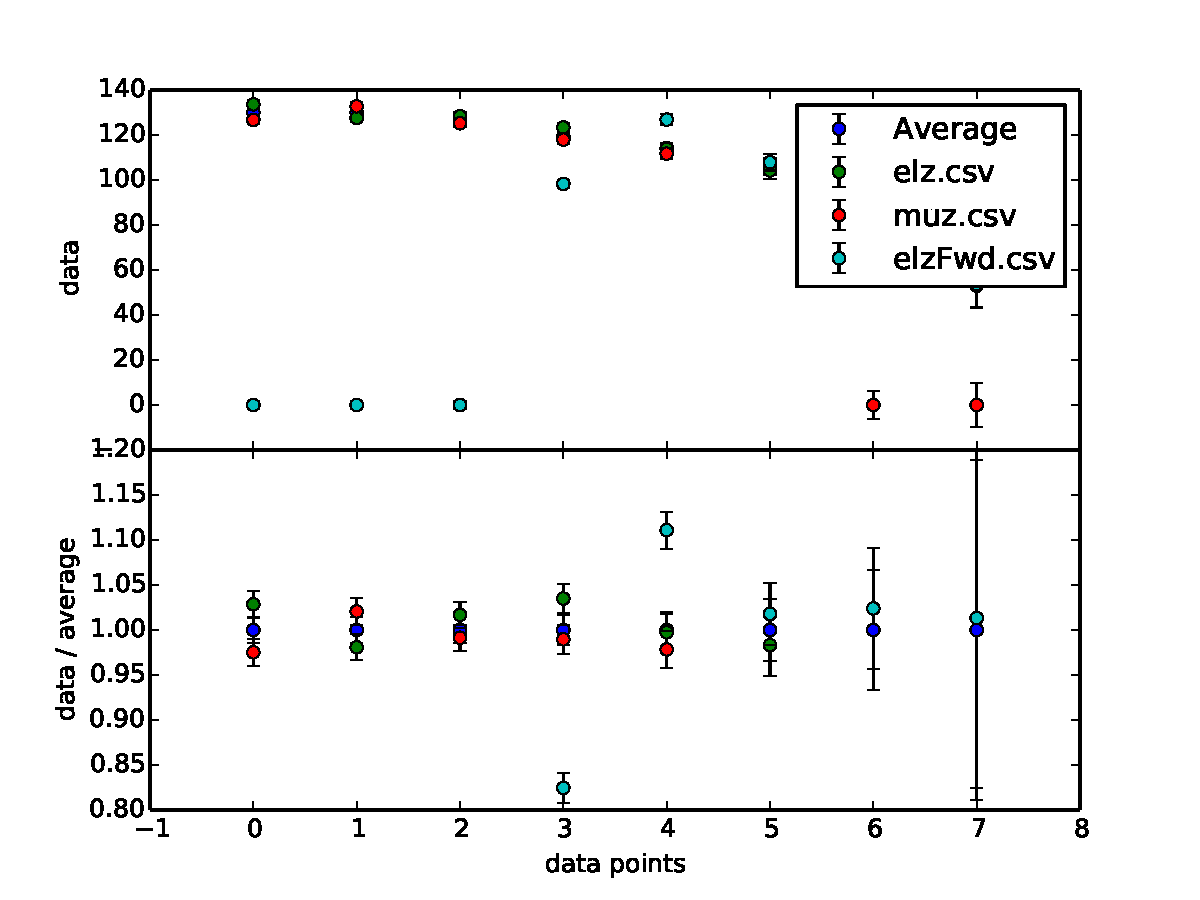
\includegraphics[width=0.49\linewidth]{figures/AvData.pdf}
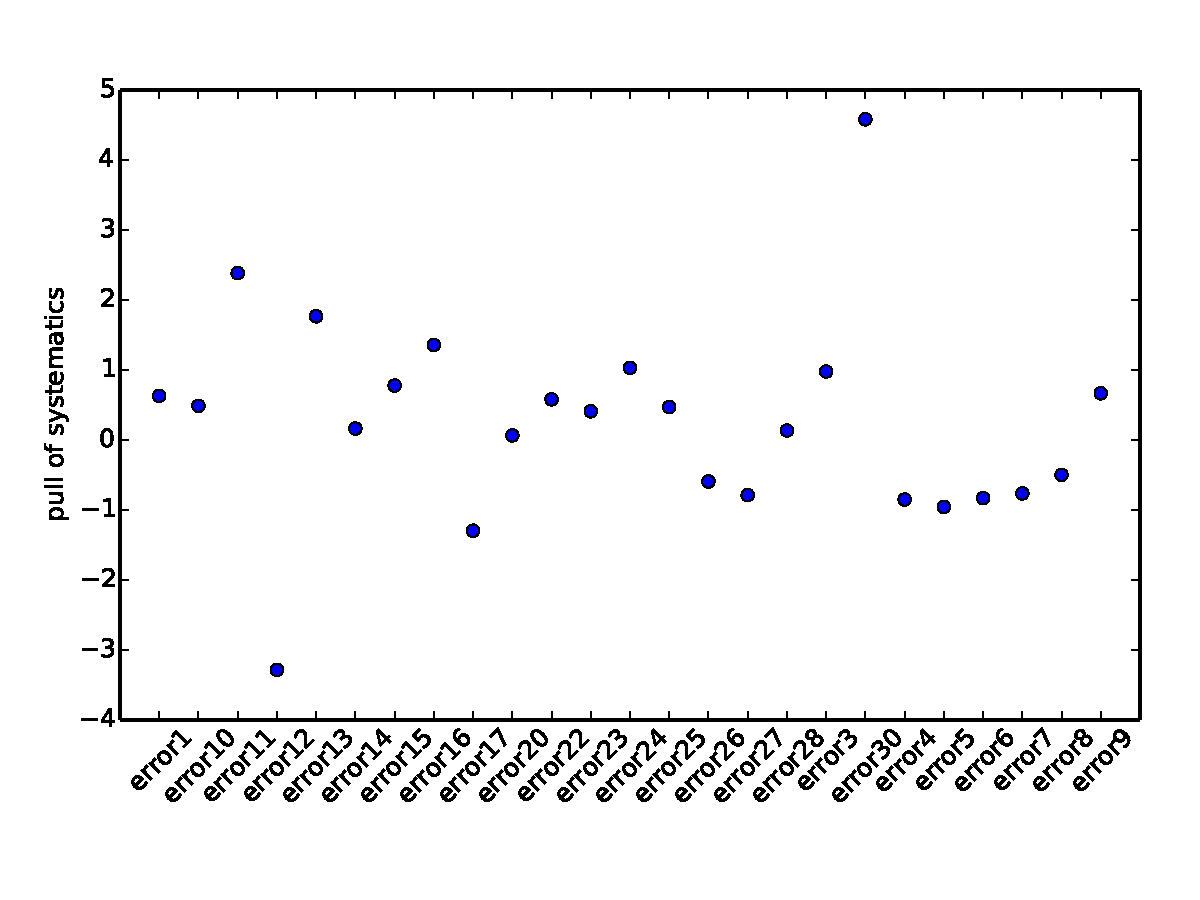
\includegraphics[width=0.49\linewidth]{figures/AvPull.pdf}

Additionally a script {\tt plot.py} plot histograms of data pulls and systematic pulls using text files as input. Therefore this script can be used also to visualise output of the fortran-base averager. Using of the script is following: 

\begin{verbatim}
./plot.py output
\end{verbatim}

where {\tt output} is the path to the output folder of the averager. This script reads files: {\tt sys.txt, tab.dat, chi2map.dat} and save plots as pdf files.


\begin{thebibliography}{99}

\bibitem{Combination}  
 A. Glazov, 
 ``Averaging of DIS cross section data,''
  AIP Conf. Proc. 792 (2005) 237--240.
  
\bibitem{HERAComb} 
H1 and ZEUS collaborations, ``Combined measurement and QCD analysis of the inclusive $e^{\pm}p$ scattering cross sections at HERA'', JHEP01 (2010) 109

\bibitem{H1Comb} 
H1 Collaboration, ``Measurement of the Inclusive ep Scattering Cross Section at Low $Q^2$ and $x$ at HERA'', Eur.\ Phys.\ J.\ C {\bf 63} (2009) 625

\bibitem{Slides} 
S. Glazov, ``Data Combination'', Statistics School, DESY, October 2011. Slides.
\end{thebibliography}

\end{document}

